\subsection{Data Description}
The training data $Xtrain$ contains 1400 observations, each 43 dimensional. One training sample has 36 real valued features and 7 categorical features. Our task is to predict the values for unseen test data, consisting in 600 samples. We measure the accuracy of our estimation using RMSE. 

\subsection{Data visualization and cleaning}
Initially, our data was not centered, as seen in $Fig.$ \ref{fig:dist_regression}.
We changed the categorical features into dummy variables, leading to a new vector of size 56. $Xtrain$ was then normalized to have 0 mean and standard deviation 1 (except the dummy variables). We applied the same operations to the test data $Xtest$ on which we will report the predicted output values.

We plotted the correlation of every feature with respect to the output and the scatter plots did not look random. We concluded the features explain the output, but we could not tell if one of them is insignificant.

The predicted values are real values in $[1000,7000]$ and seemed to be grouped into two blobs. We believed initially the smaller blob represented outliers, but since it contained almost $10\%$ of the data we decided not to ignore it.

After looking at every feature individually, we noticed that feature 36 offers a clear separation of the two blobs (see $Fig.$ \ref{fig:feature36}). We therefore chose to fit two models, one in which feature 36 has values greater than $-13$ and one in which it is smaller, corresponding to smaller predicted values. We will refer to the points grouped to the left of the black vertical line in $Fig.$ \ref{fig:feature36} as the first blob or big blob model and the points to the right as the small blob.


\begin{figure}[ht]
  \centering
  \begin{subfigure}[b]{0.45\textwidth}
   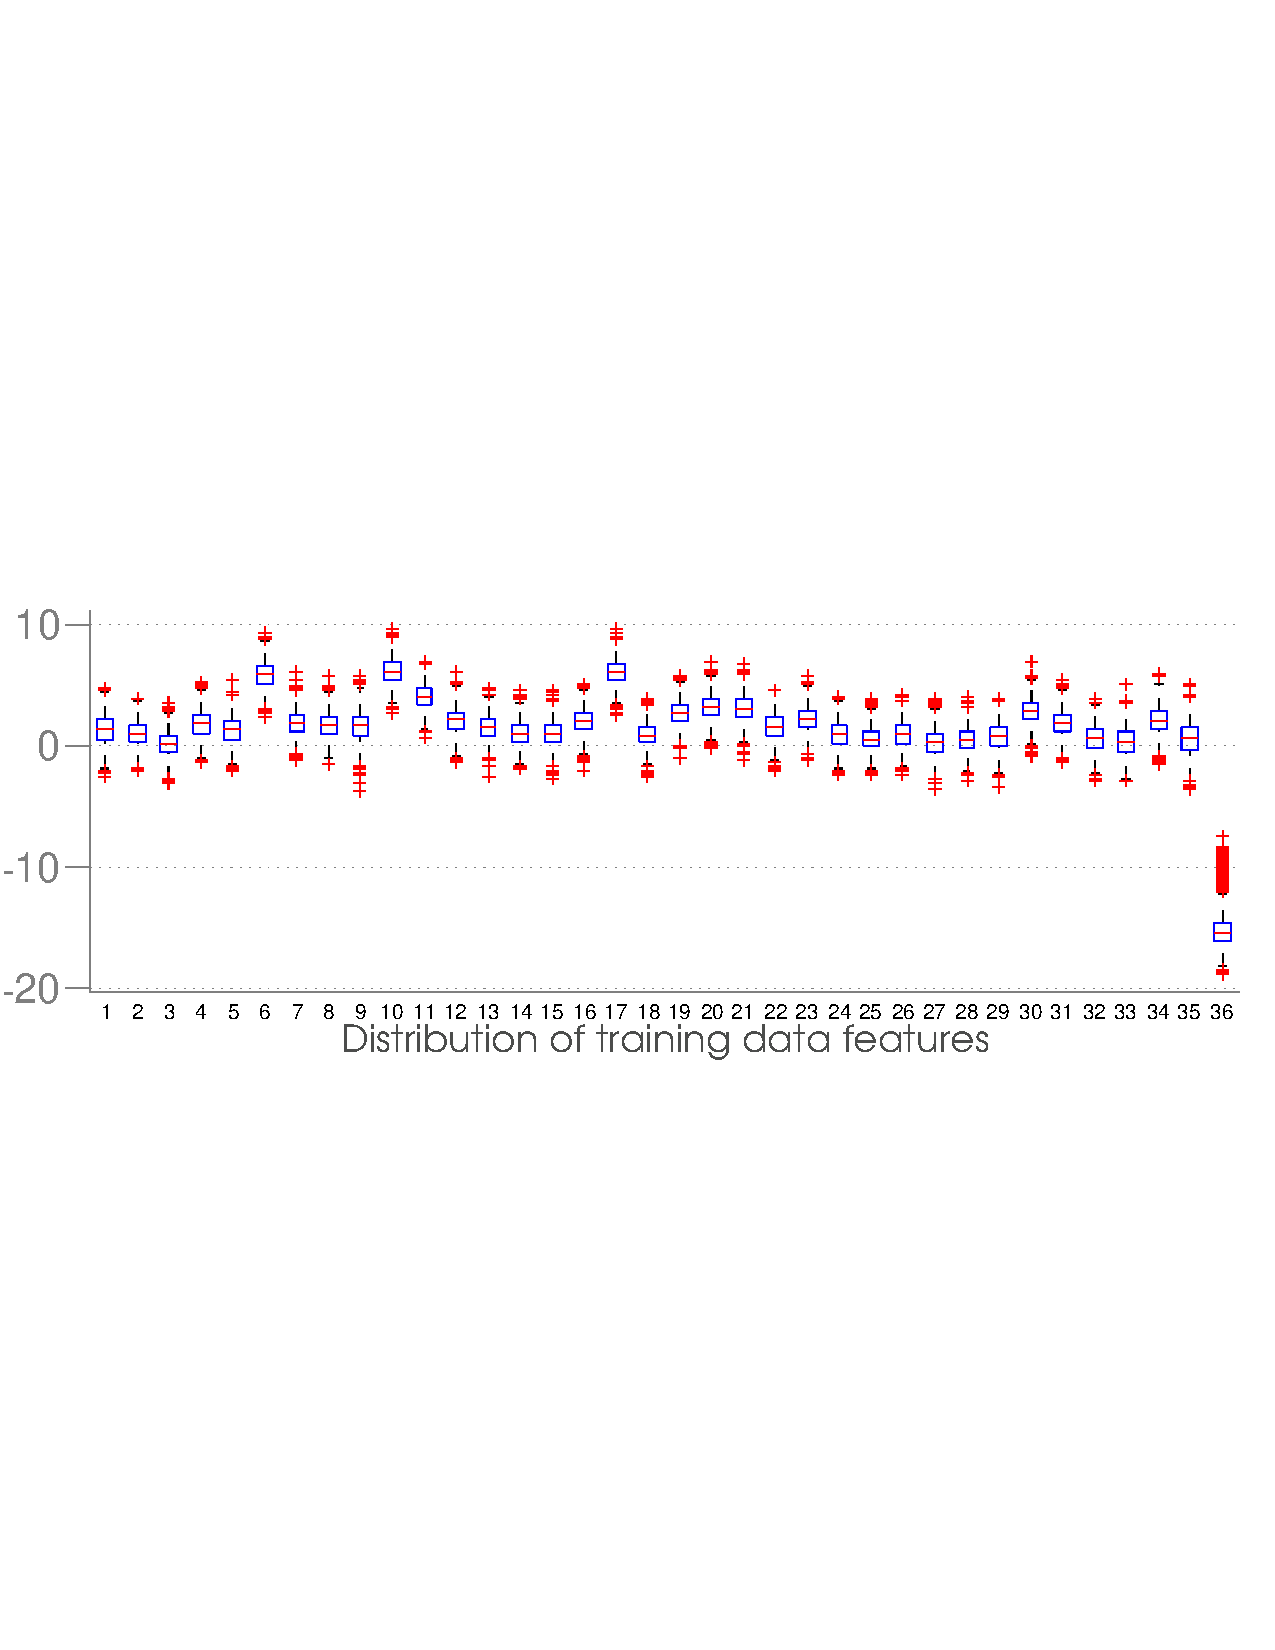
\includegraphics[width=0.45\textwidth]{figures/distribution_regression_crop.pdf}
    \caption{Mean and standard deviation for the first 36 real valued variables of Xtrain. The input is not normalised and feature 36 is the only negative one.}
    \label{fig:dist_regression}
  \end{subfigure}
  \begin{subfigure}[b]{0.45\textwidth}
    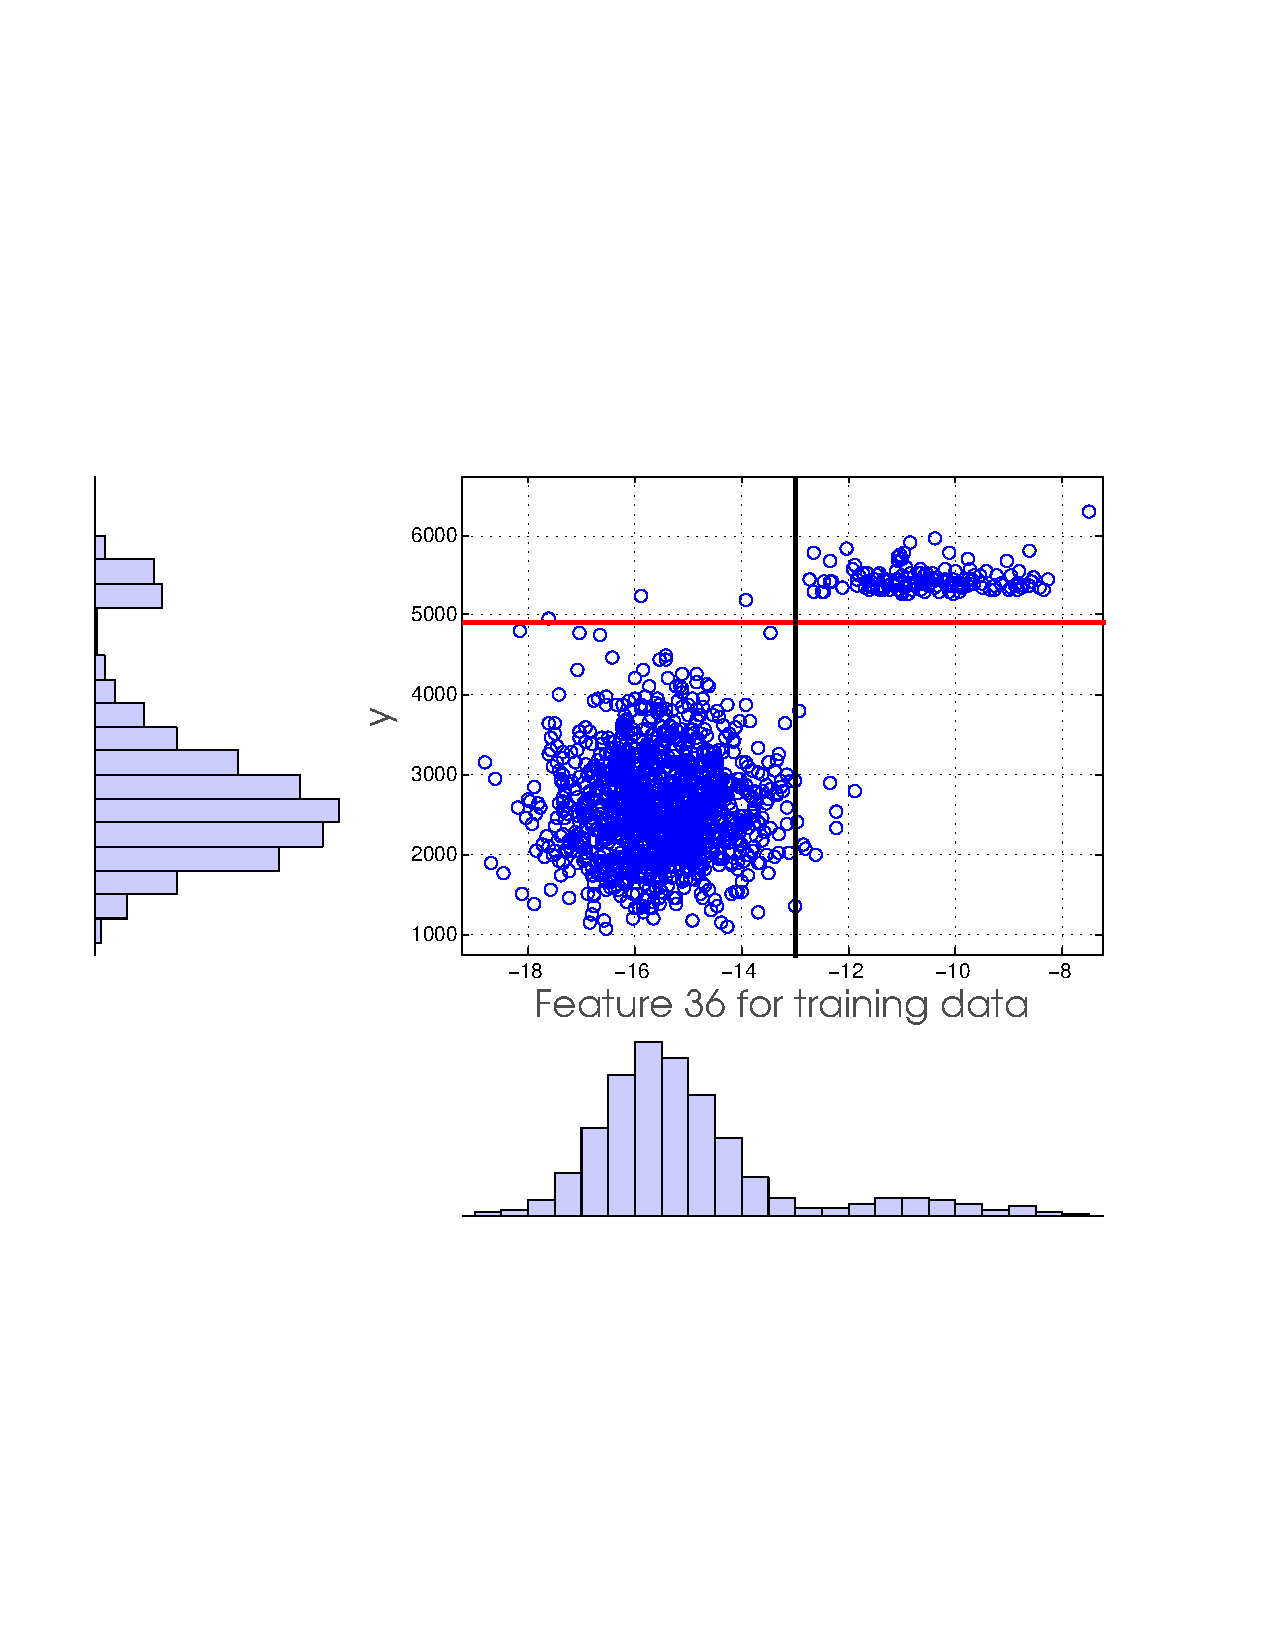
\includegraphics[width=0.45\textwidth]{figures/feature36_13_crop.pdf}
    \caption{Feature 36 versus output values. X = 1.4 (black line) and y = 4900 (red line)  provide a good separation of the two blobs.}
    \label{fig:feature36}
  \end{subfigure}
  \caption{Data visualization}
\end{figure}

We visually observed some linear correlations between certain features such as feature 2 and 24, 13 and 16, 17 and 20, but we decided to keep them since we did not have time to experiment with their removal or to test their significance. This is corroborated by the fact that $Xtrain$ is rank deficient, it has 57 columns after the use of dummy variables but rank 50.

If the input is normally distributed with mean 0 and standard deviation 1, then
 $99.99\%$ of the samples appear between the values -3.891 and 3.891. We therefore remove any points that are outside this interval, considering them outliers.

\subsection{Regression baseline methods}
After the visualization and the analysis of the data, we applied to them the regression methods that we had implemented. More specifically, we used the least squares method (developed both using the normal equations and gradient descent) and the ridge regression method. All of them produced results of similar quality, fact that may be confirmed by the almost equal RMSE for training and test data parts, but also by the values of their resulting $beta$, which are pretty close to each other.

The following analysis, except the part of parameters computation, is referred to the results obtained from the ridge regression, but could be generalized to all of the above mentioned methods. In all of the experiments 80\% of the data are used for the training part and 20\% of them are used for the test part. Furthermore, K-fold cross-validation  with $K=5$ is used to obtain the error presented at this section.

$Figures$ \ref{fig:alpha1} and \ref{fig:alpha2} present the results of the experiments that were held in order to find the best value of the parameter $\alpha$ for the least squares using gradient descent method. For this experiments 50 values of alpha that range between $10^{-3}$ and 0.2 were used. As we can observe, for both of our models when $\alpha$ has small value the RMSE that is produced is higher. The error decreases as the value of $\alpha$ increases up to the value 0.04. After this the performance of the method (regarding RMSE) is similar for all of the values of the parameter.

\begin{figure}[ht]
  \centering
  \begin{subfigure}[b]{0.45\textwidth}
   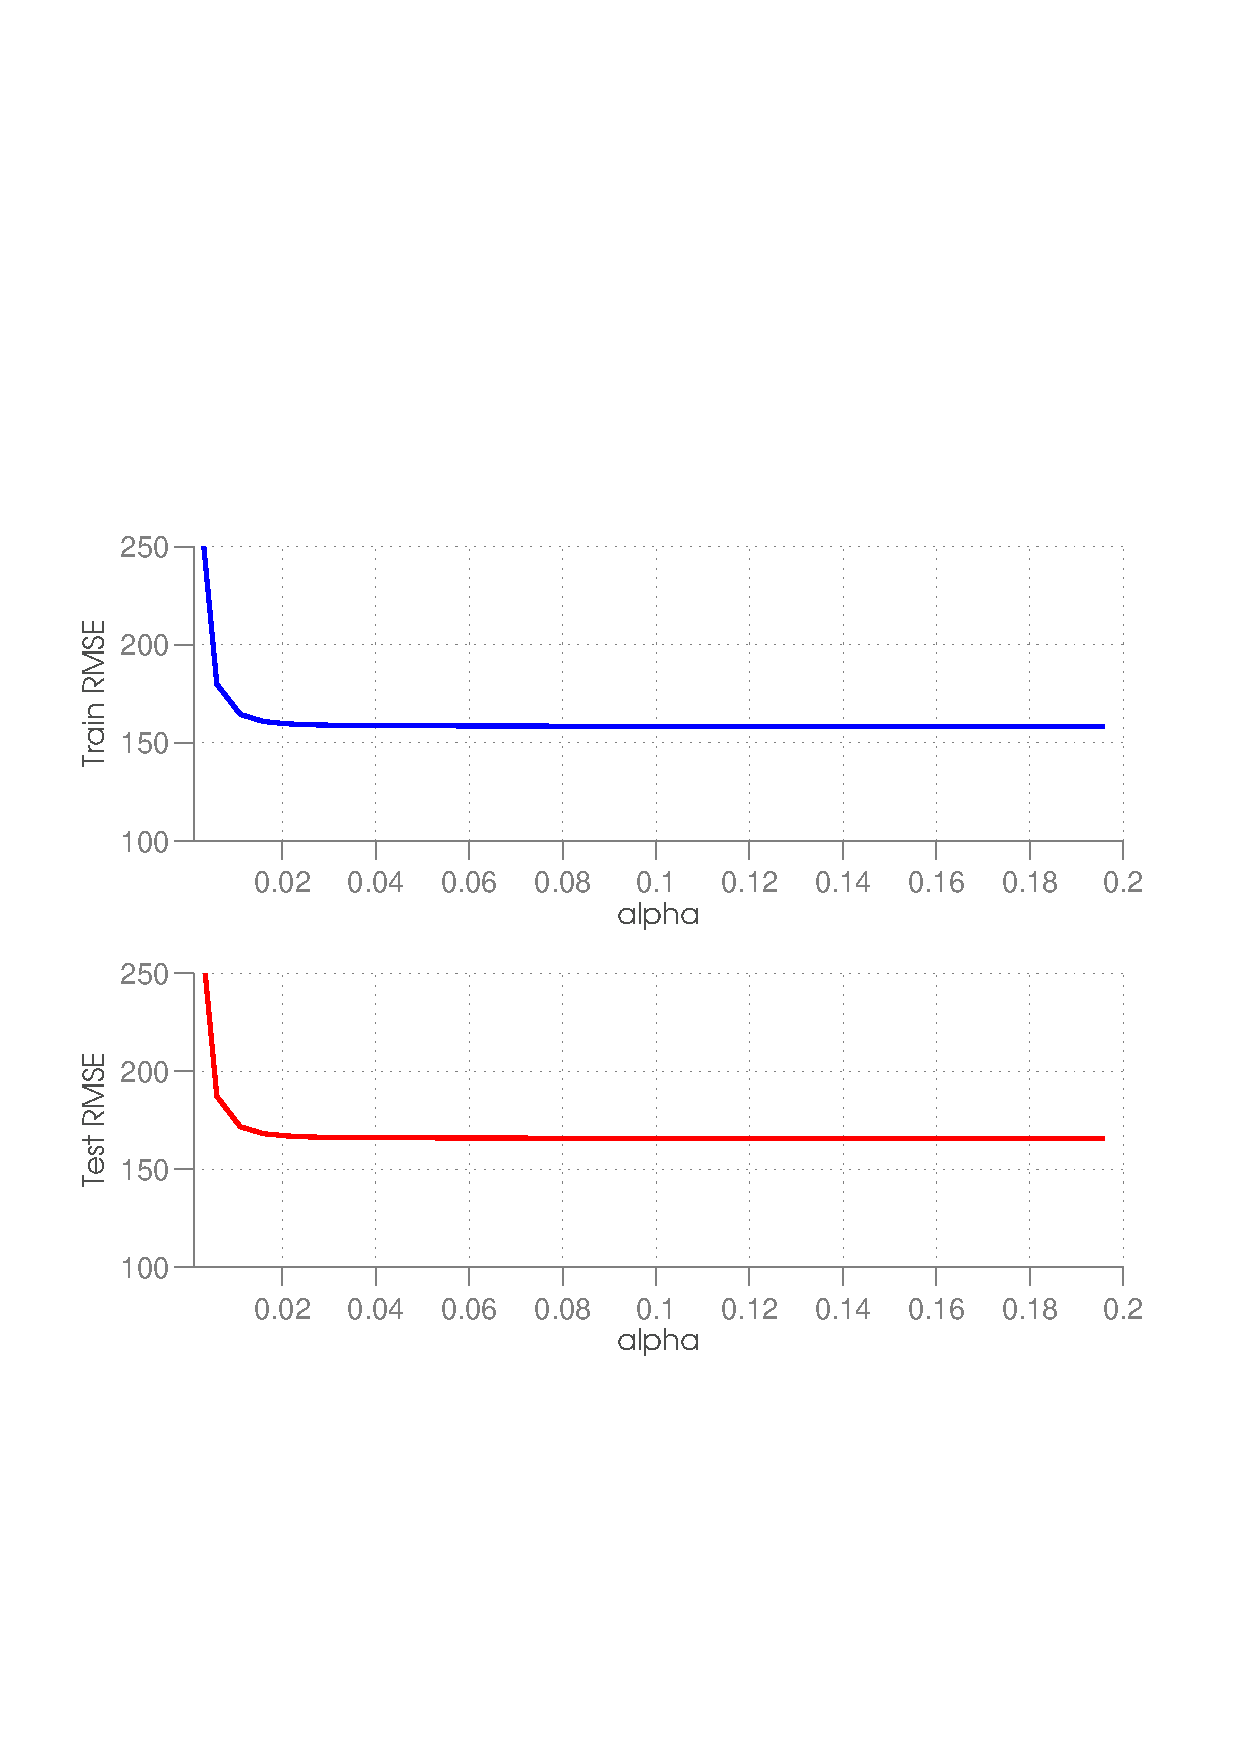
\includegraphics[width=\textwidth]{figures/alpha_curve1.pdf}
    \caption{Results for the big blob.}
    \label{fig:alpha1}
  \end{subfigure}
  \begin{subfigure}[b]{0.45\textwidth}
    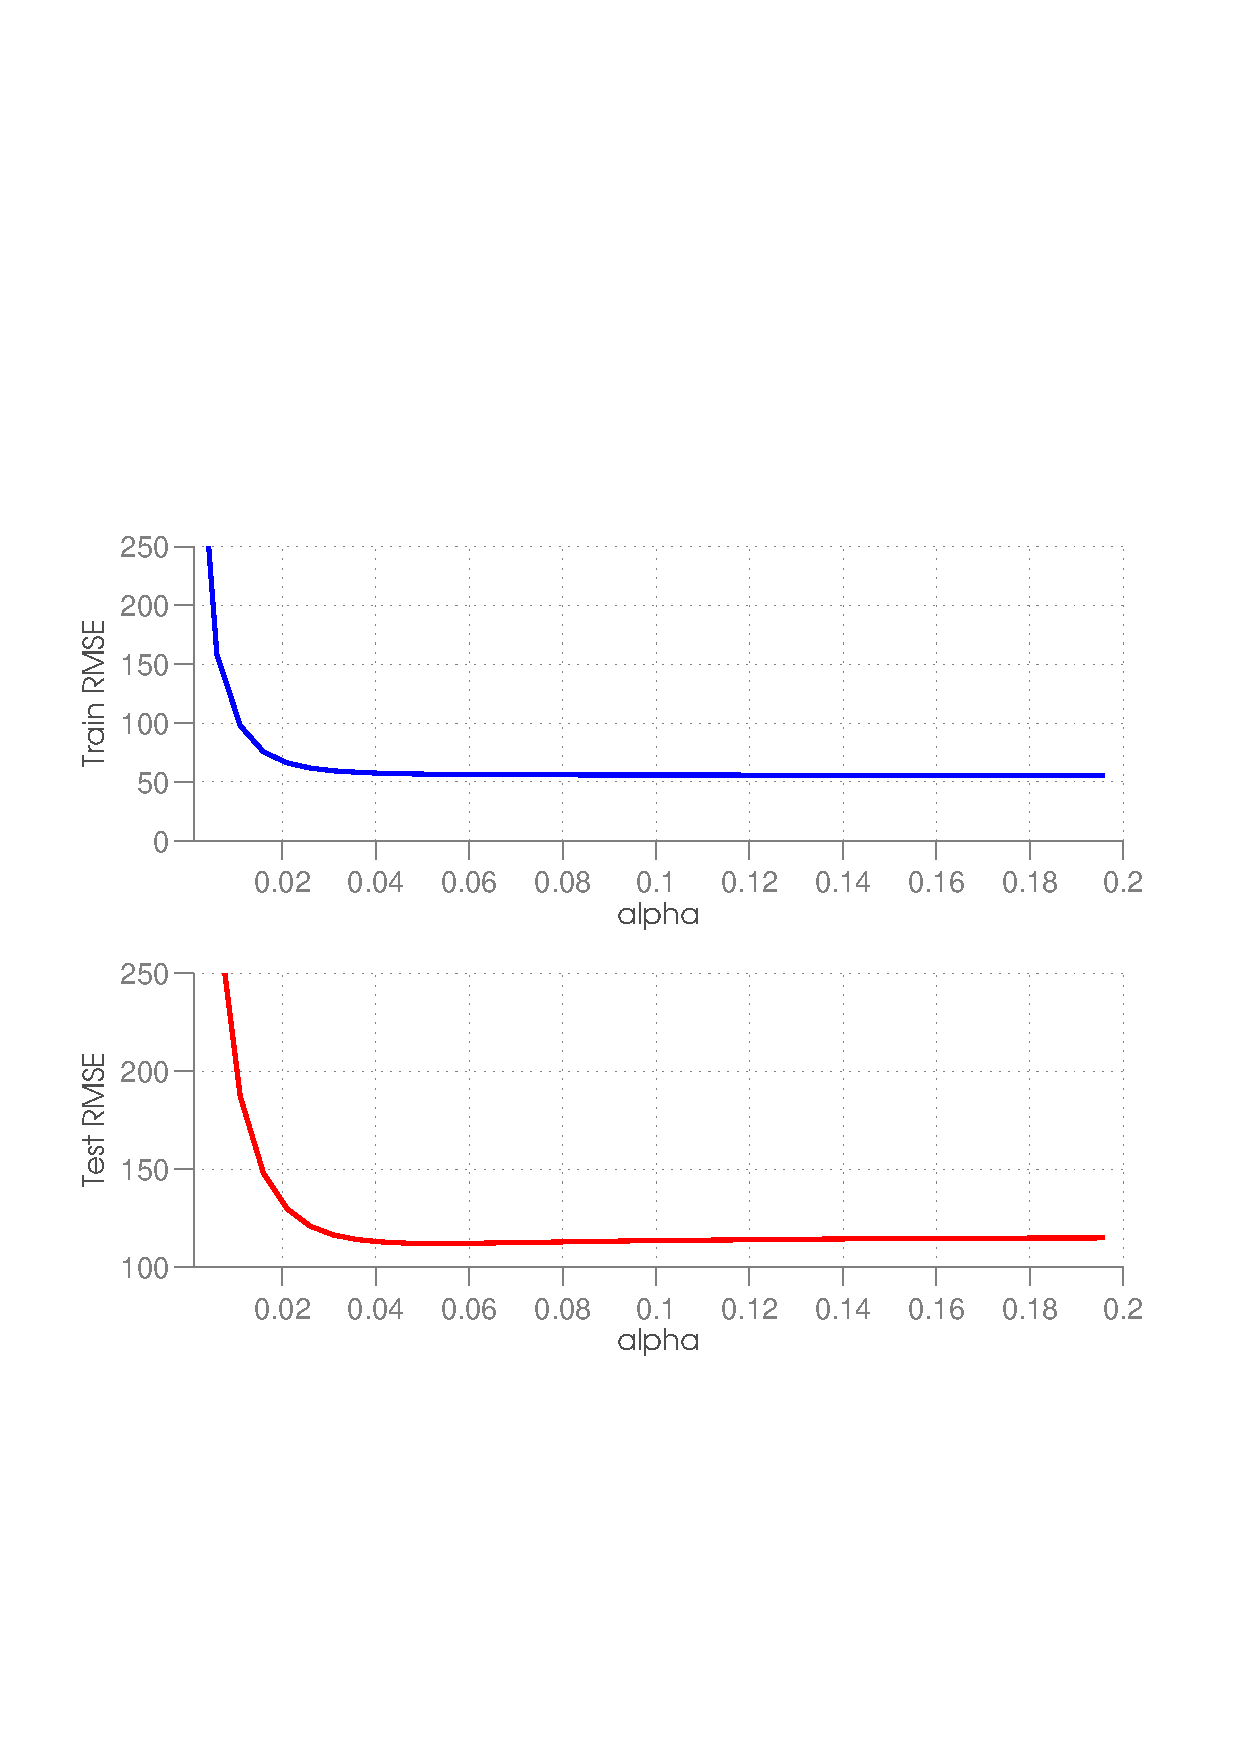
\includegraphics[width=\textwidth]{figures/alpha_curve2.pdf}
    \caption{Results for small blob.}
    \label{fig:alpha2}
  \end{subfigure}
  \caption{RMSE produced for 50 values of $\alpha$ ranging between $10^{-3}$ and 0.2. Results refer to both b fitted by least squares using gradient descent.}
\end{figure}

Regarding the ridge regression method we used 1000 different values for $\lambda$ between $10^{-7}$ and 0.1. As in all of our cases 80\% of the data was used for the training and the rest was reserved for the validation. $Figures$ \ref{fig:lambda1} and \ref{fig:lambda2} show the results, where we can see that when $\lambda$ increases the RMSE grows, too. This makes us to choose a very small $\lambda$ for our experiments. Moreover, the fact that our model performs better for very small values $\lambda$, makes ridge regression very close to least squares, regarding its behaviour. That is one more evidence that the two methods perform similarly to our data, as we mentioned above.

\begin{figure}[ht]
  \centering
  \begin{subfigure}[b]{0.45\textwidth}
   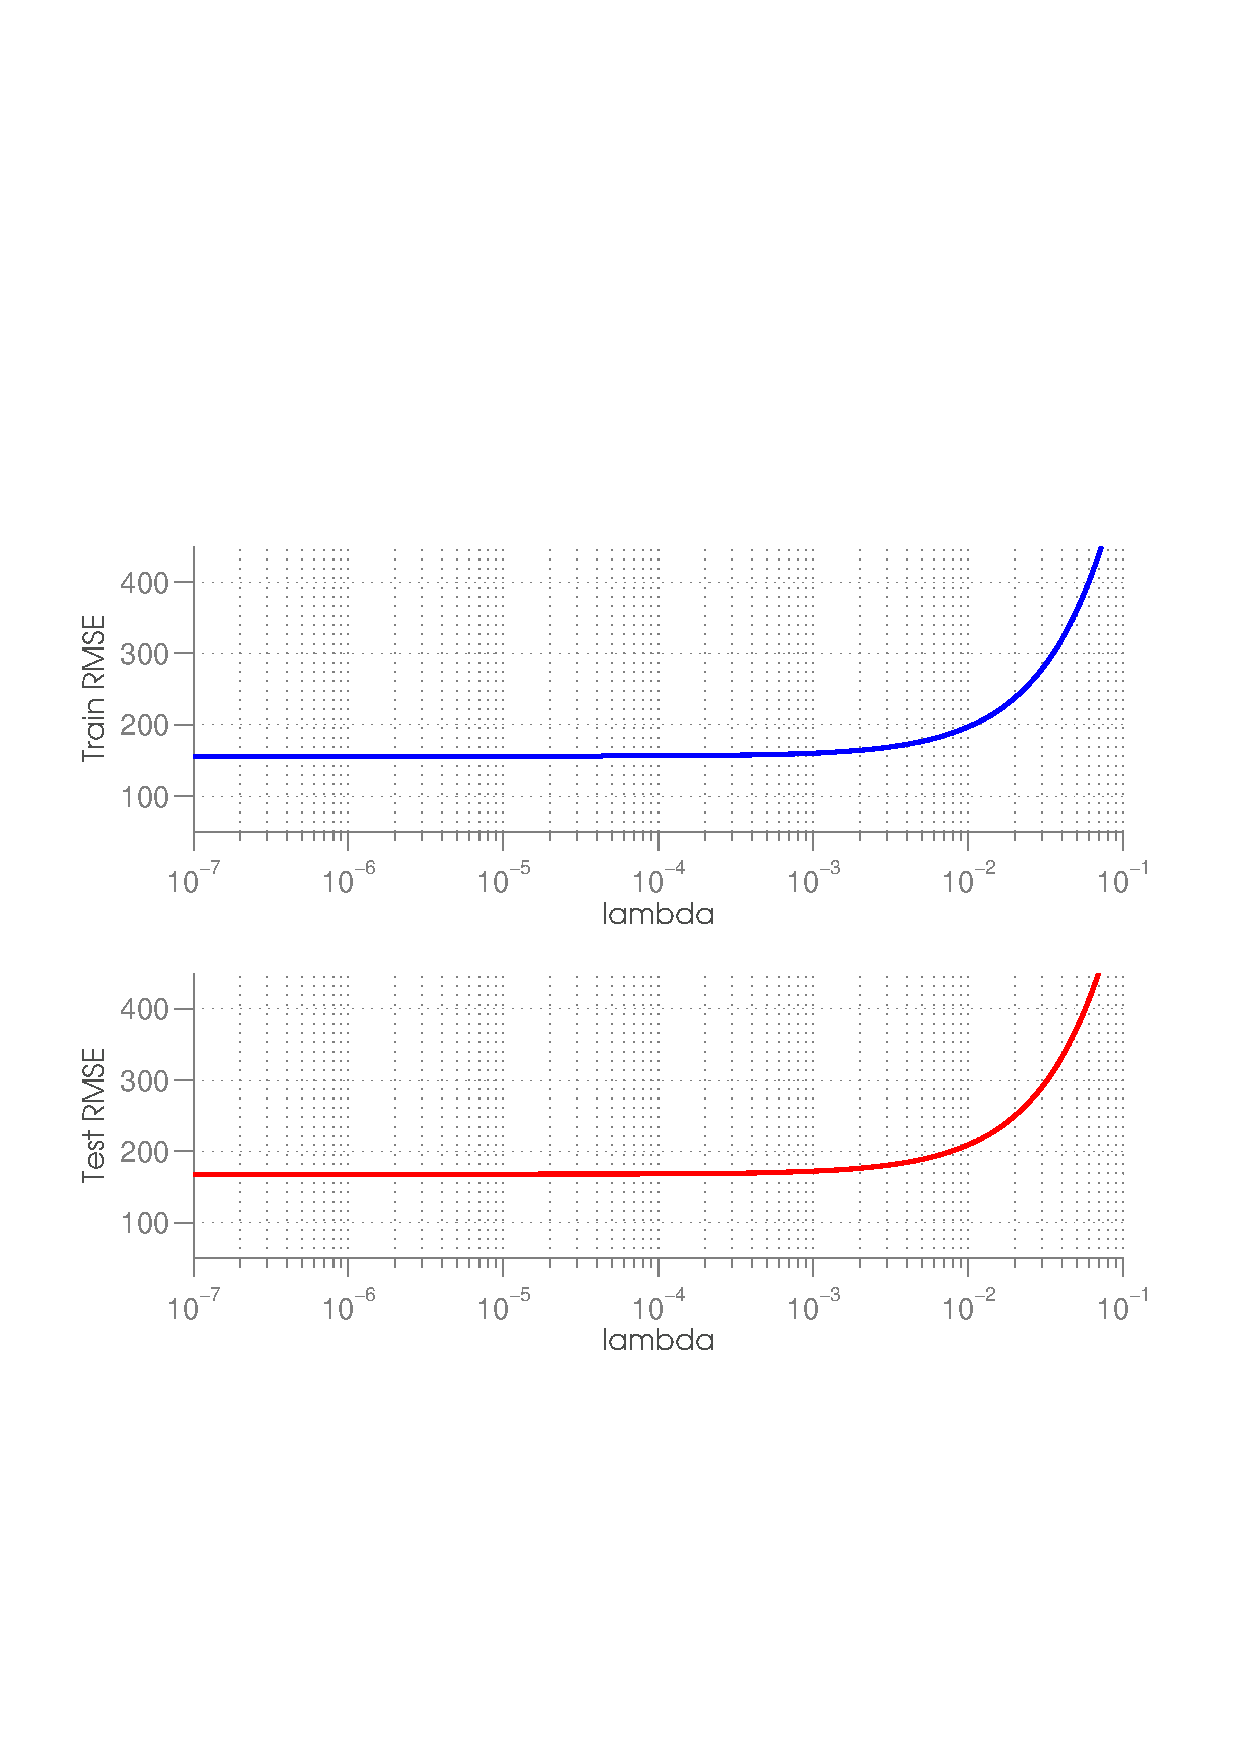
\includegraphics[width=\textwidth]{figures/lambda_curve1.pdf}
    \caption{Results for the big blob.}
    \label{fig:lambda1}
  \end{subfigure}
  \begin{subfigure}[b]{0.45\textwidth}
    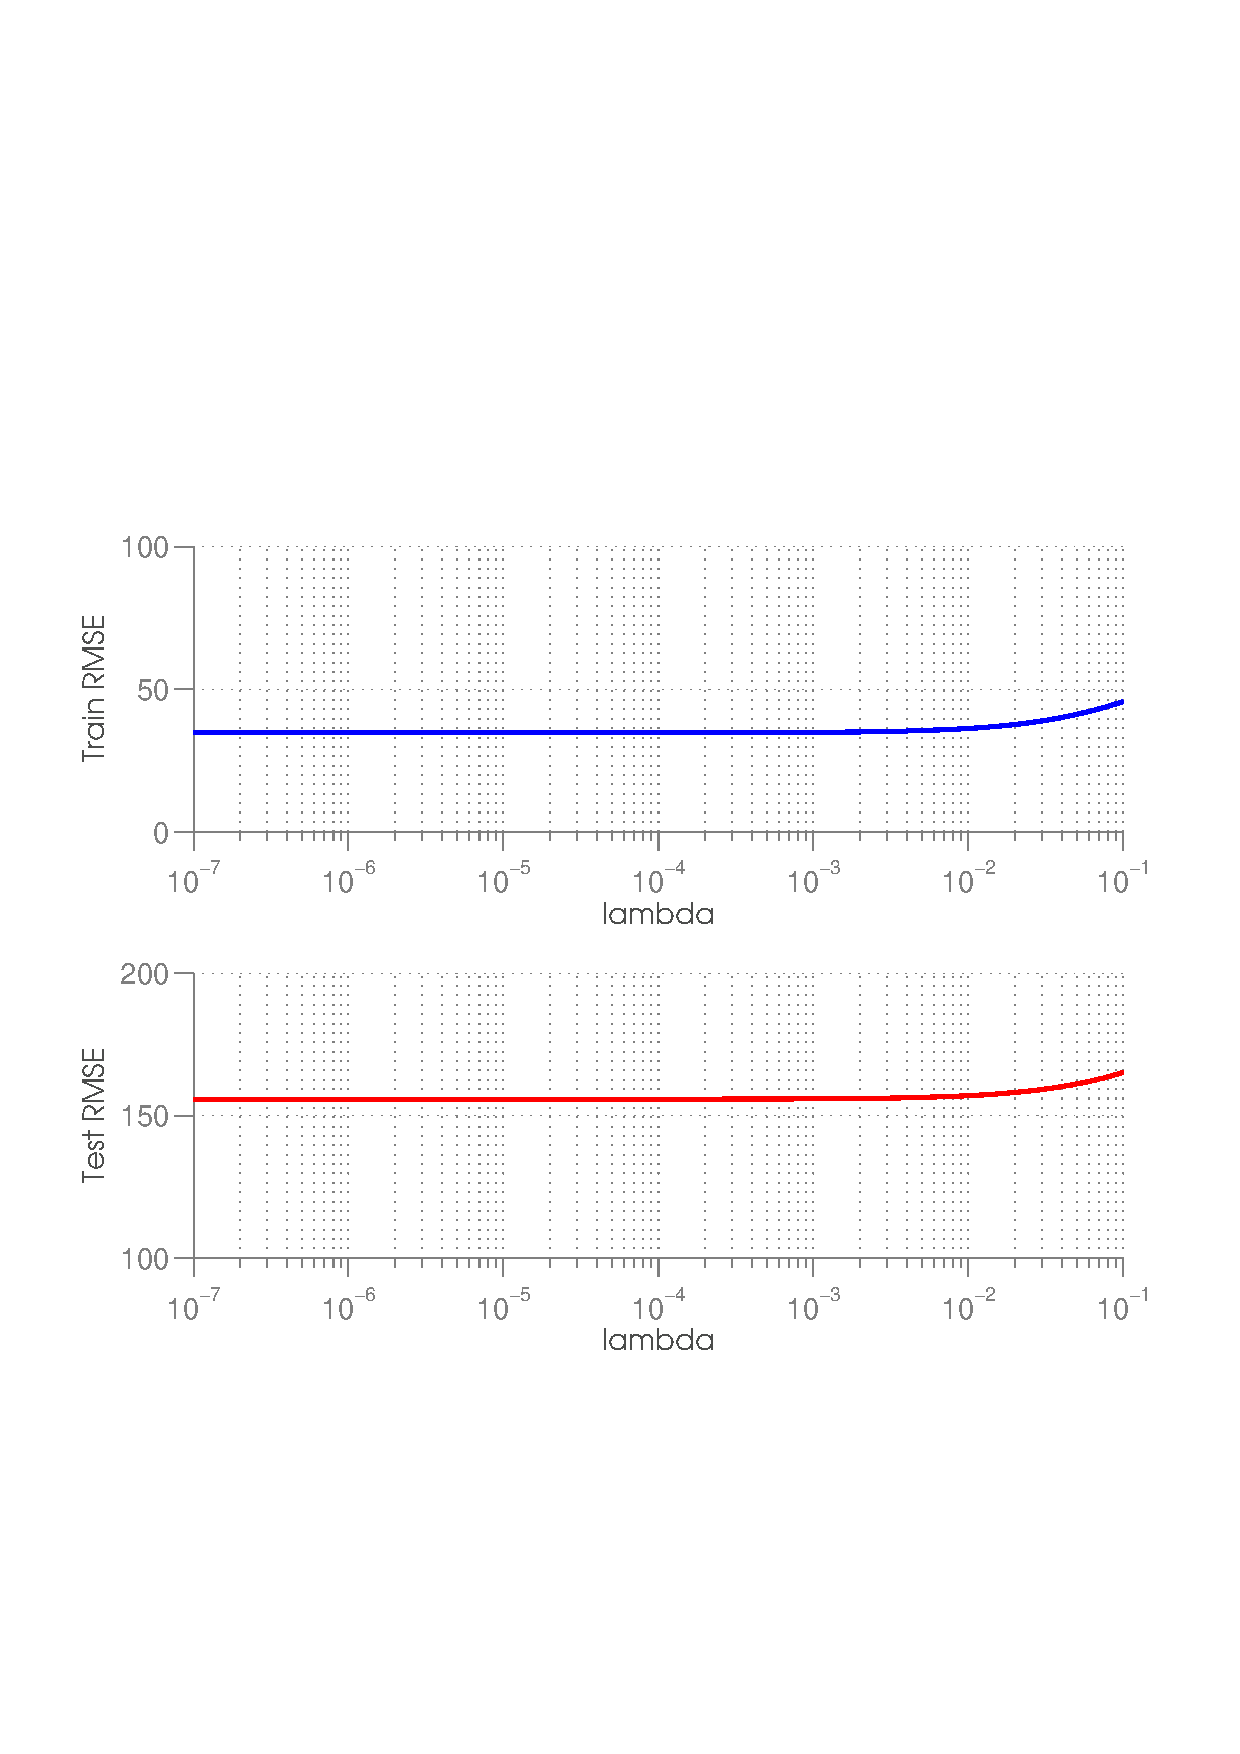
\includegraphics[width=\textwidth]{figures/lambda_curve2.pdf}
    \caption{Results for small blob.}
    \label{fig:lambda2}
  \end{subfigure}
  \caption{RMSE produced for 1000 values of $\lambda$ ranging between $10^{-7}$ and 0.1. Results refer to both models fitted by ridge regression.}
\end{figure}

For the last part of this section's experiments we tried to study how the amount of the data that are used for training affects the resulting errors. We kept a constant amount of the data (20\% of the given) for the training and we used the rest of them in proportional way for training. We started using 10\% of the training part for our training and we continued up to 100\%. Each experiment was held 50 times with 50 different randomly selected subgroups of data and the results shown represent the average of these experiments.

$Figure$ \ref{fig:learning_curve} presents the RMSE obtained for the two models, after using each proportion of the training data. As we can see, when the proportion increases the RMSE for training and the RMSE for validation tend to some specific values.

\begin{figure}[ht]
  \centering
   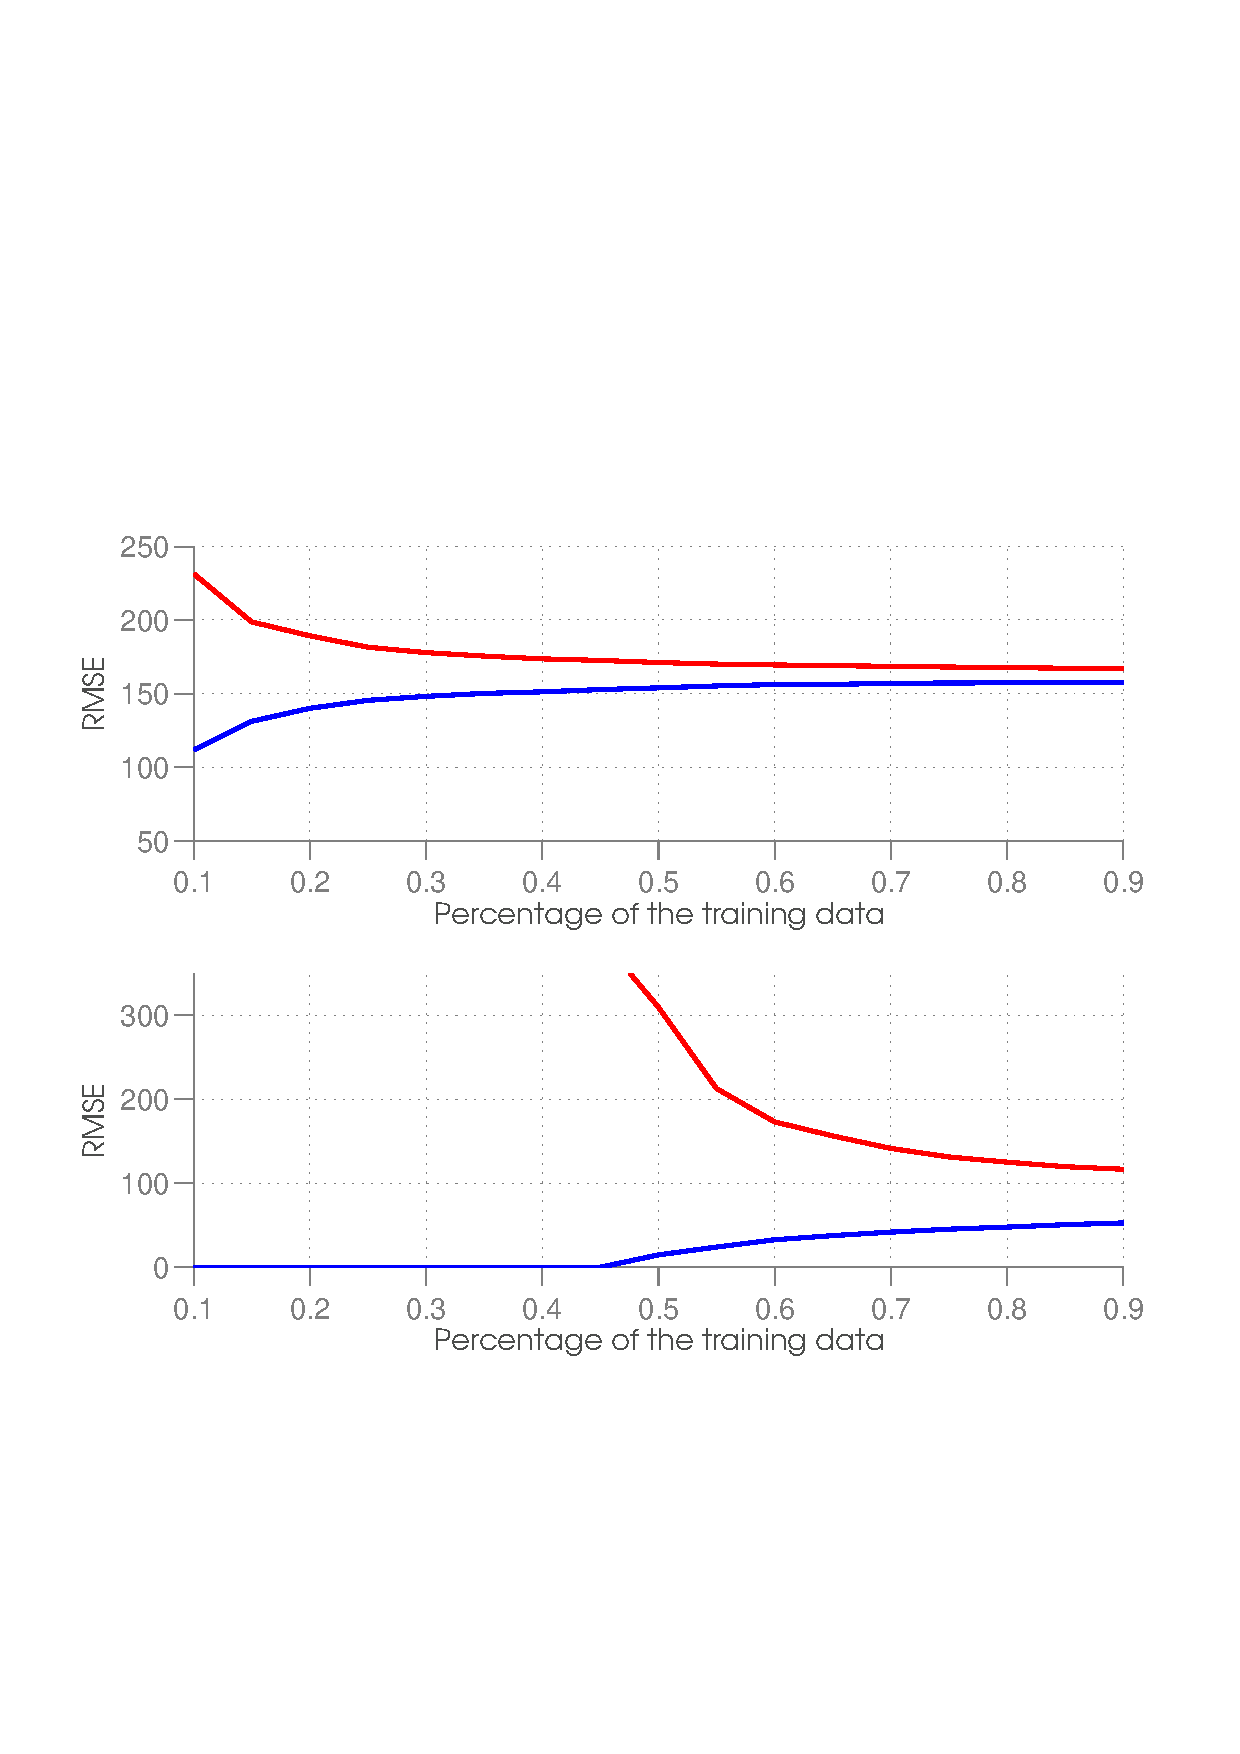
\includegraphics[scale=0.45]{figures/learning_curve.pdf}
    \label{fig:learning_curve}
  \caption{Learning curve produced for our model using ridge regression. The blue lines represents the train RMSE and the red the test RMSE. Moreover, the top figure represents the big blob and the bottom figure the small blob.}
\end{figure}

\subsection{Feature transformations}
We tried polynomial and exponential transformations of the features.
The exponential transformation did not prove to work well and we focused on polynomial regression.
We only transformed the first 36 variables and kept the categorical variables as they are since polynomial transformation of categorical variables does not have an intuitive interpretation. 

In all our experiments we used 5-fold cross-validation. The degree of the polynomial was varied from 1 to 10 for both blob-models. In $Fig$ \ref{fig:degree_blob1}, \ref{fig:degre_blob2} we plotted the mean training and validation RMSE for the degree varying only between 2 - 10 and 2 - 6 respectively for readability (for the other values the RMSE was too big). 

We tried both $\lambda$ and $\alpha$ with values in the set $\{10^i | i =-5,...,2\}$.
Using 5-fold cross validation with $\lambda = 10{-7}, \alpha = 0.1$ we
notice that a polynomial of degree 3 is the best fit for the first blob. Increasing it further leads to over-fitting, since the training errors becomes very small and the validation error increases. For the second blob model, using  $\lambda = 0.001, \alpha = 0.1$ we obtain a best fit for a polynomial of degree 2.

\begin{figure}[h]
  \centering
  \begin{subfigure}[b]{0.45\textwidth}
   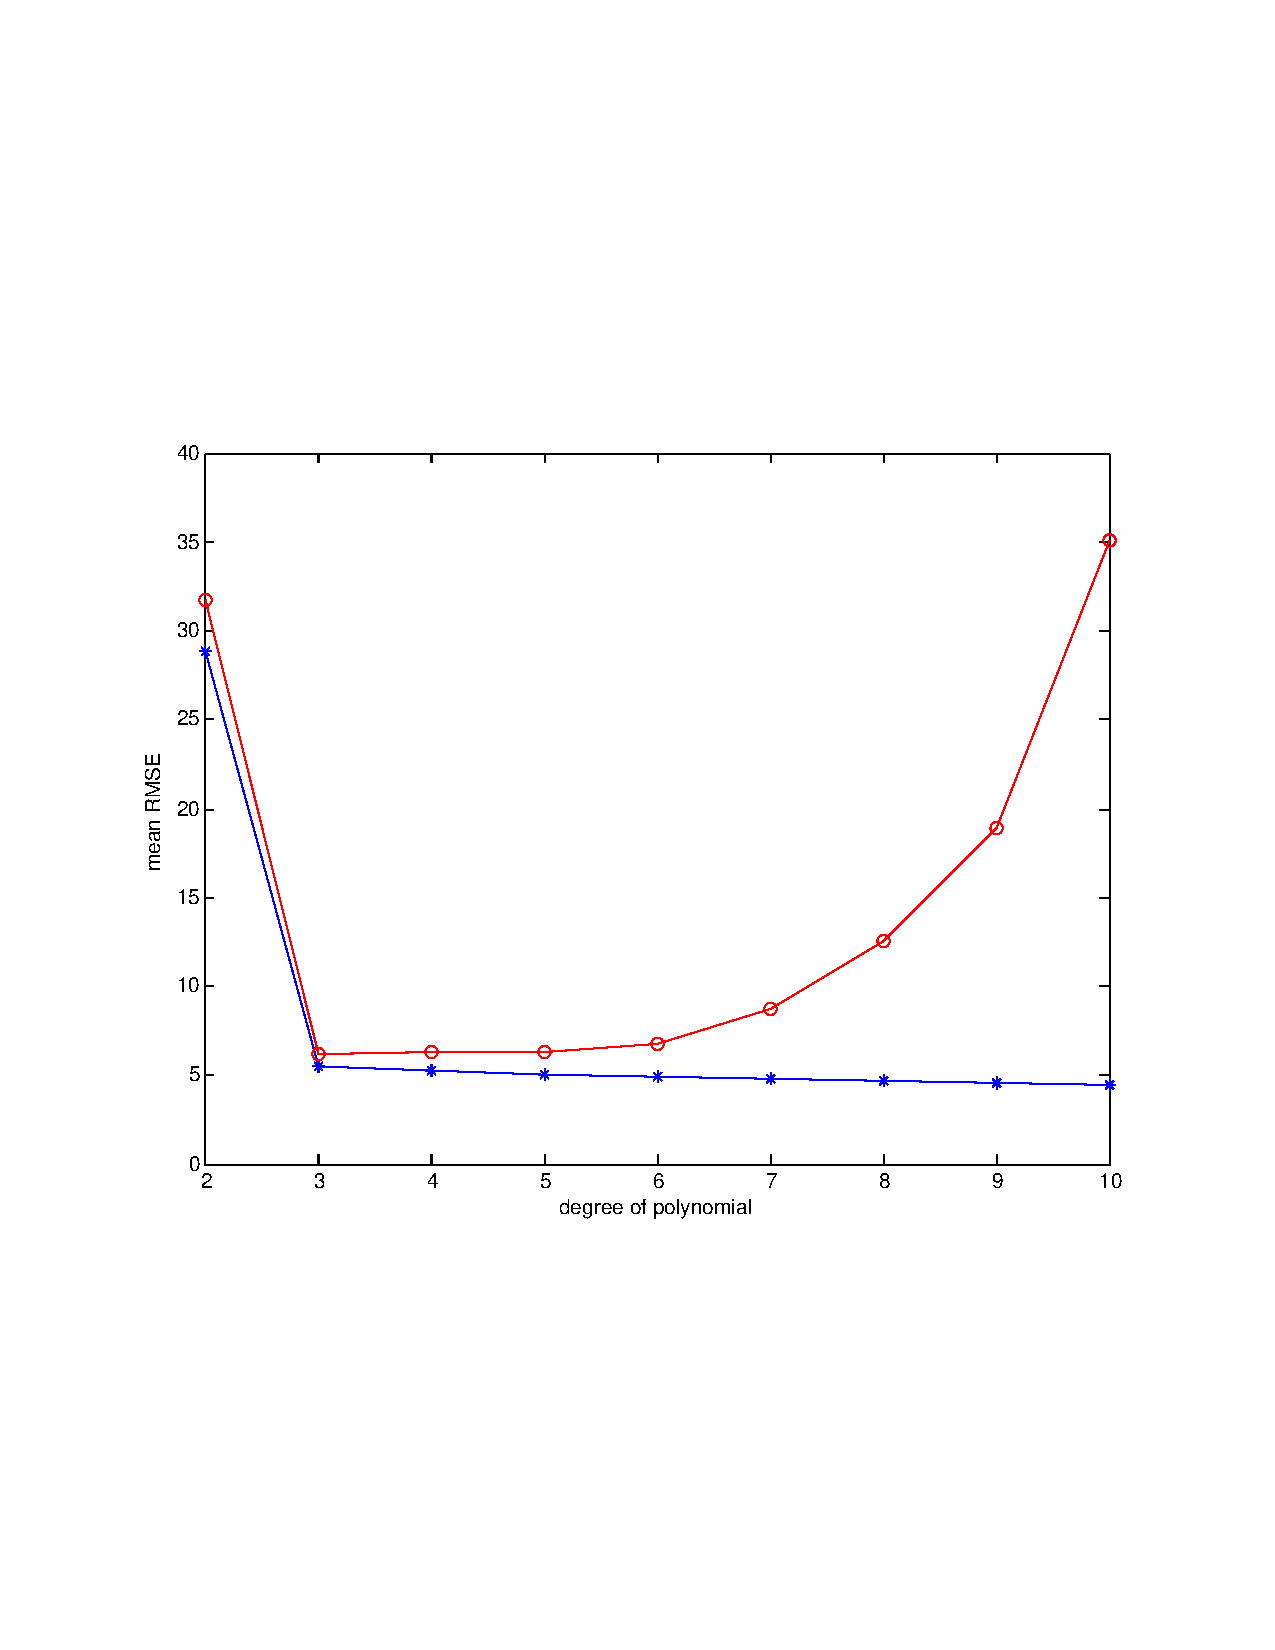
\includegraphics[width=\textwidth]{figures/degree_polynomial_blob1_crop.pdf}
    \caption{First Blob. Mean RMSE for training set \newline (blue curve) and testing (red curve) versus poly-\newline nomial degree. The errors were computed using\newline 5-fold cross-validation.}
    \label{fig:degree_blob1}
  \end{subfigure}
  \begin{subfigure}[b]{0.45\textwidth}
    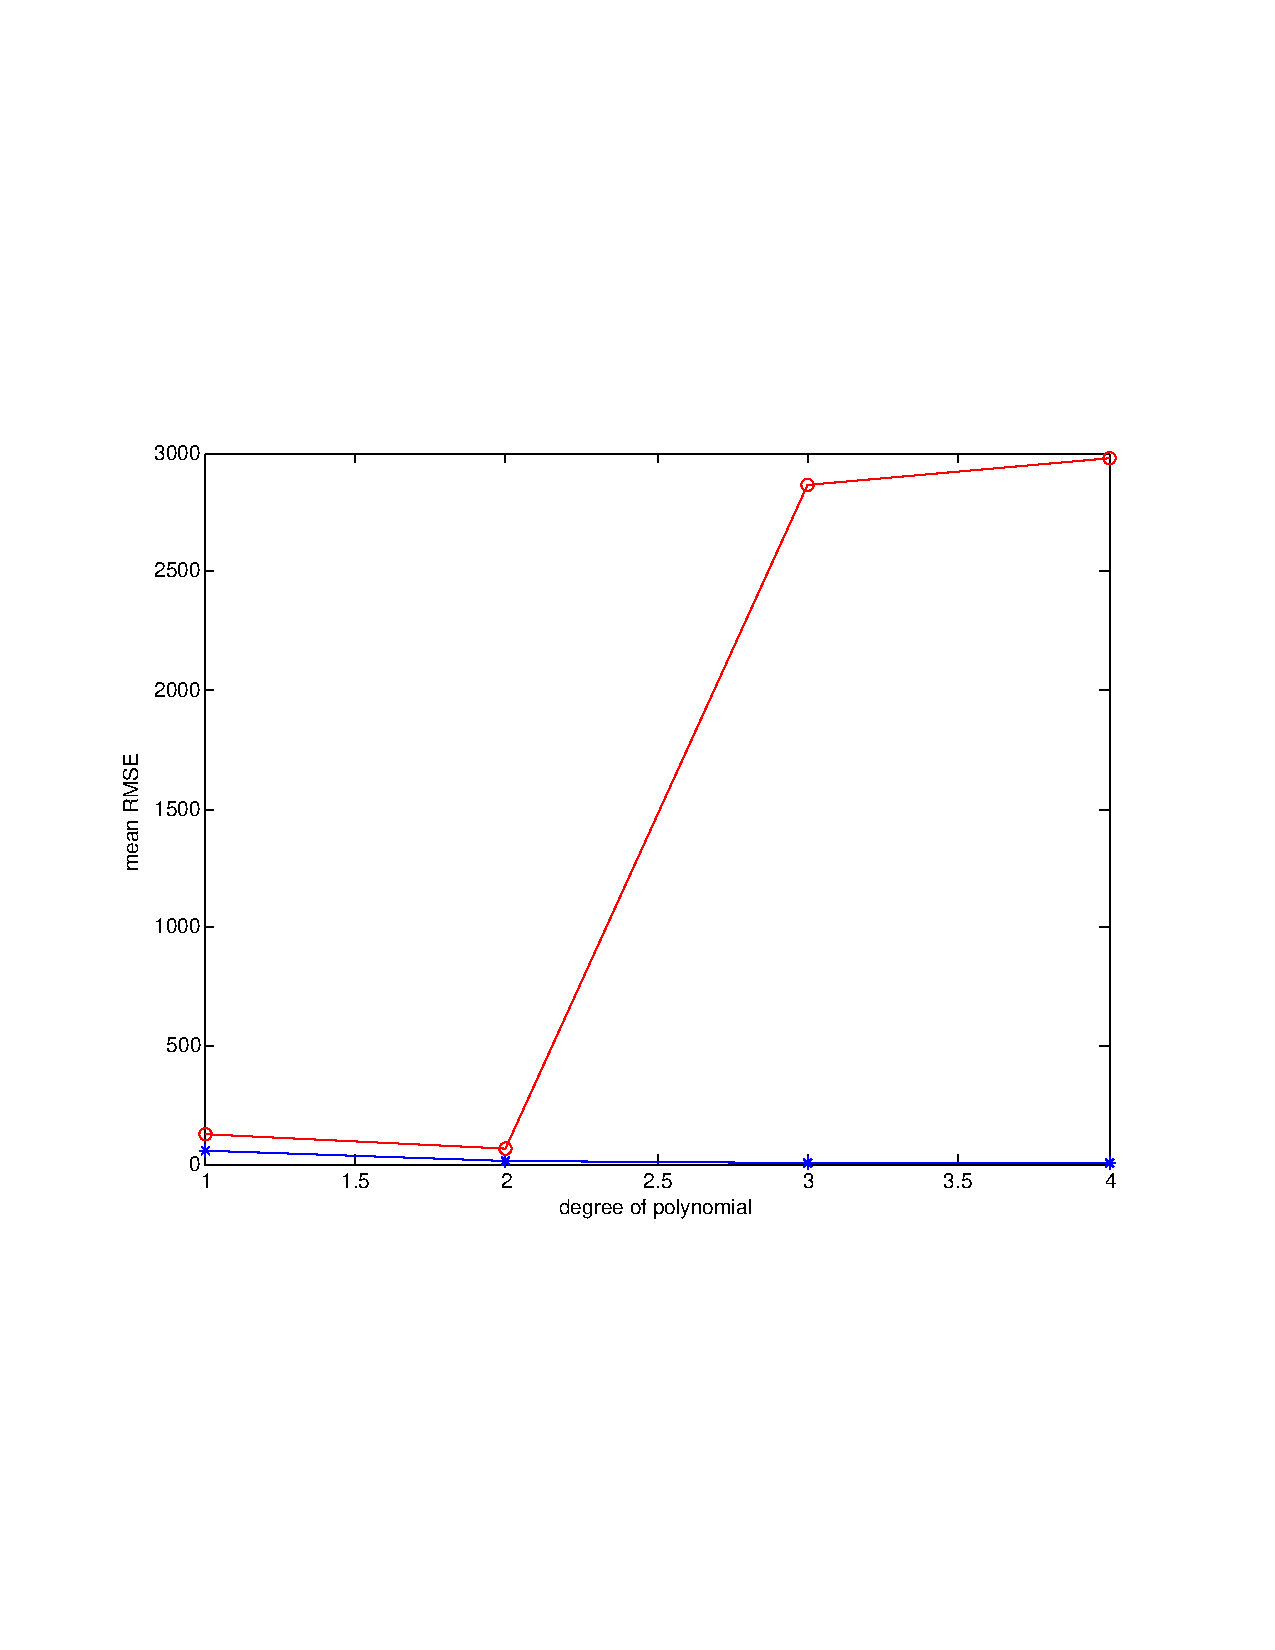
\includegraphics[width=\textwidth]{figures/degree_polynomial_blob2_crop.pdf}
    \caption{Second Blob. Mean RMSE for training set (blue curve) and testing (red curve) versus polynomial degree. The errors were computed using 5-fold cross-validation.}
    \label{fig:degre_blob2}
  \end{subfigure}
  \caption{Selection of polynomial degree}
\end{figure}

We increased lambda to prevent over-fitting, since we have 10 times less samples for the second model. However, we still noticed that our RMSE for the validation set was  bigger for the second blob. This might be due to the fact that we have a very small set for both training and testing of the second model.

Both polynomial regression models significantly outperform the normal ridge regression, which gave a RMSE greater than 100. Table \ref{table:feat_transform} summarizes our best results. We notice that for the first model, our training and testing errors were quite similar and the standard deviation was quite small. For the second model, the validation error was much bigger than the train error, which is an indicate of over-fitting. 

\begin{center}
  \begin{tabular}{ |l | c | c| }
    \hline
     & RMSE train & RMSE test \\ \hline
    Blob1 model & 5.37 ($\pm$ 0.044) & 6.25 ($\pm$ 0.4) \\ \hline
    Blob2 model & 7.16 ($\pm$ 1.85) & 58.10 ($\pm$ 16.2) \\
    \hline
  \end{tabular}
  	\label{table:feat_transform}
    \captionof{table}{Estimated Train and Test RMSE for the two blob models.}
\end{center}

We note that our assumption that in our training set we have a clear separation between the two blobs using the value of feature 36 is not a realistic approximation. The problem is that there are some samples with feature 36 less than -13 whose predicted value should be estimated using model 1 and some which should use model 2. This can also be seen in $Fig.$ \ref{fig:feature36}.
Because of this, we expect our error on new unseen data to be big for samples that have feature 36 value in the range $[-12,-14]$.
 
To test this, we split $Xtrain$ into $20\%$ for testing and $80\%$ for training and validation. We applied the same data processing as before, we estimated model parameters as above and the RMSE per model proved to be very similar with the ones in Table \ref{table:feat_transform}. 

However, as we expected, our test error on the held out $20\%$ got much worse. The total RMSE for our $20\%$  test data was 295.78 (RMSE= 73.5 for blob 1, RMSE = 887.24 for blob 2 and 295.78 RMSE combined).
If we remove all the samples in the held out test data which have feature 36 in the interval [-12,-14], we obtain a total RMSE = 68.62 (RMSE = 71.6 for model 1, RMSE = 82.77 for model 2). We see that the bad fit for blob 2 decreased and it is now comparable with the one from blob 1. This validates our hypothesis that high error values come from that part of the model. To sum up, we have two models that work well separately but perform bad for samples with feature 36 near the threshold value.

Our model is a piecewise polynomial and can suffer from various problems. Since we do not enforce continuity at the 36th feature, our model will generate high errors for samples that have the value of feature 36 near the threshold value, in our case -13. This happens because feature 36 does not give a clear separation of the data into two distinct models. A possible solution for further research would be to enforce smoothness at the thresholded value.

\subsection{Summary}
For the regression section we performed experiments on the given data using least squares and ridge regression methods. All of them have pretty similar results considering the produced RMSE. The test error estimation considering both blobs is 160.233.

The feature transformations that were introduced seemed to improve the results, decreasing the errors, but a more careful approach shows that the models that are produced very probably over-fit the data.